\newpage\subsection*{1551 Worksheet 3 Answers}

\SolutionsStatement

\begin{enumerate}
	
    \item (b) is the only correct expression. Don't forget that $\log_a(x) + \log_a(y) = \log_a(xy)$, and $\log_a(x) + \log_a(y) \ne \log_a(x + y)$.
    
    \item \begin{enumerate} 
    \item For example,     $$g(x) = \begin{array}{cc}
    \begin{cases}
      \ x , & 0 \le x < 1 \\
      \ \frac{1}{x - 1} , & x \ge 1 \\
    \end{cases}
    \end{array}$$
    \item There are many possible solutions. For example, $$f(x) = \begin{array}{cc}
    \begin{cases}
      \ x , & 0 \le x < 1 \\
      \ 2 , & x \ge 1 \\
    \end{cases}
    \end{array}$$
    Or you could use $f(x) = \frac{|x|}{x}$.
    \end{enumerate}
    
    \item \begin{enumerate}
    \item False. Counterexample: $$f(x) = \begin{array}{cc}
    \begin{cases}
      \ x , & 0 \le x < 1 \\
      \ 2 , & x \ge 1 \\
    \end{cases}
    \end{array}$$
    \item False. The domain of $\ln x$ is $(0,\infty)$, so $e^{\ln x} = x$ only for $x > 0$.
    \end{enumerate}
    \item $f$ is a continuous function, $f(0) > 0$, $f(1) < 0$. By the intermediate value theorem, there is a value of $x \in [0,1]$ such that $f(x) = 0$. 
    
    \item For $g$ to be continuous at $x = 1$, we need $\lim_{x \rightarrow 10^+} g(x) = \lim_{x \rightarrow 10^-} g(x)$. We can compute both limits, set them equal, and solve for $a$. 
    \begin{align*}
    	\lim_{x \rightarrow 10^+} g(x) &= a - 10 \\
        \lim_{x \rightarrow 10^-} g(x) &= 3 \\
        \Rightarrow a - 10 & = 3 
        \Rightarrow a = 13
    \end{align*}
    
        \begin{center}
    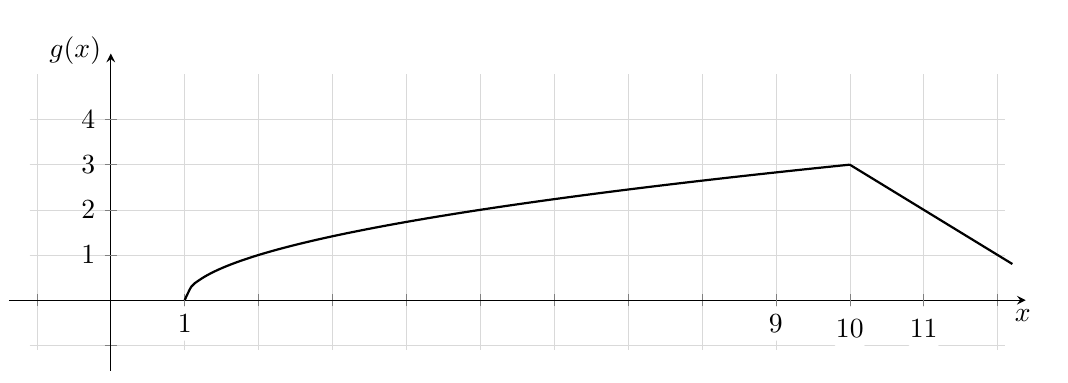
\begin{tikzpicture}[domain=-1:11] 
        \begin{axis}[
        width=5.5in,
        height=2in,
        grid=both,
        grid style={line width=.2pt, draw=gray!30},
        clip=false,
        axis lines=middle,
        xmin=-1.1,xmax=12.1,
        ymin=-1.1,ymax=5,
        restrict y to domain=-1:4,
        xtick={-2,-1,0,1,...,9,10,11,12},
        xticklabels={, , , , , , , , , ,},
        ytick={-1,0,1,2,3,4},
        yticklabels={, , , , , , , , , ,},
        extra x ticks={1,9,10,11},
        extra y ticks={1,2,3,4},
        extra x tick style={xticklabel style={fill=white, circle, inner sep=1.5pt}},
        extra y tick style={xticklabel style={fill=white, circle, inner sep=1.5pt}},
        extra x tick labels={1,9,10,11},
        extra y tick labels={1,2,3,4},
        axis line style={shorten >=-7.5pt, shorten <=-7.5pt},
        xlabel=$x$,
        ylabel=$g(x)$,
        xlabel style={at={(ticklabel* cs:1)},anchor=north west},
        ylabel style={at={(ticklabel* cs:1)},anchor=south east}
        ]
        \addplot[samples=100,domain=1:10,smooth, thick] {sqrt(x-1)} node[pos=1] (endofplotsquare) {};  
        \addplot[samples=100,domain=10:12.2,smooth, thick] {13-x} node[pos=1] (endofplotsquare) {};  
        \end{axis}
    \end{tikzpicture} 
    \end{center}
    
    \item Evaluate the following limits.
    \begin{enumerate}
    	\item \begin{align*} 
        \lim_{x \rightarrow 0^-} \frac 1 x - \frac{1}{|x|} 
        &= \lim_{x \rightarrow 0^-} \frac 1 x + \frac{1}{x} = -\infty
        \end{align*}
        This one-sided limit does not exist (DNE). 
    	\item Apply the sandwich (or squeeze) theorem. 
        \begin{align*} 
        	-x^2 \le x^2\sin\left(\frac{1}{x^4}\right) \le x^2\\
        	\lim_{x \rightarrow 0} -x^2 = \lim_{x \rightarrow 0} +x^2 = 0 \\
        	\Rightarrow \lim_{x \rightarrow 0} x^2\sin\left(\frac{1}{x^4}\right) = 0
        \end{align*}
    	\item 
        \begin{align*} 
         	\lim_{x \rightarrow 2} \frac{\frac 1 x - \frac 1 2}{x^2 - 4} 
            & =\lim_{x \rightarrow 2} \frac{\frac {2}{2x} - \frac {x}{2x}}{(x-2)(x+2)} \\
            & =\lim_{x \rightarrow 2} \frac {1}{2x} \frac{2 - x}{(x-2)(x+2)} \\
            & =\lim_{x \rightarrow 2} \frac {1}{2x} \frac{-(x-2)}{(x-2)(x+2)} \\
            & =\lim_{x \rightarrow 2} \frac{-1}{2x(x+2)} \\
            &= \frac{-1}{16}
		\end{align*}
    \end{enumerate}    
    
\end{enumerate}




